\subsection{React}
\label{reactjs}
React ist eine der beliebtesten JavaScript Frameworks zum Erstellen von sogenannten 
Single-Page-Apps. React beschreibt sich selbst als JavaScript Bibliothek und nicht wie andere als 
ein Framework. React ist viel mehr eine Anleitung, wie man verschieden Dinge machen könnte.
React ist also kein All-in-One Paket.


Reacts Entwicklungsgrund war es eine möglichst performante Oberfläche zu gestalten. Dabei werden 
einfache Views erstellt und React übernimmt die Änderung der Daten innerhalb der View. React 
erstellt einen sogenannten virtuellen DOM bei der Datenanzeige.


\begin{figure}[H]
  \begin{center}
    
\includegraphics[width=0.1\textwidth]{Theorie/React/React-icon.svg.png}
    \caption{ReactJS Logo~\cite{reactjs}}
  \end{center}
\end{figure}

\subsubsection{Virtuelles DOM}
VDOM ist ein Programmierkonzept, bei dem durch den Prozess \textit{Reconciliation} eine ideale, 
virtuelle Darstellung der Benutzeroberfläche im Speicher gehalten wird und mit dem realen DOM durch 
eine Bibliothek wie ReactDOM synchronisiert wird. Dies ermöglicht eine deklarative API von React, 
bei der man den Zustand der Benutzeroberfläche angibt und React stellt sicher, dass das DOM diesem 
Zustand entspricht. Dies entfernt verschiedene Arbeitsschritte, welche sie sonst durchführen müssten.
VDOM ist viel mehr ein Muster als eine spezifische Technologie. Der Begriff virtuelles DOM wird in 
React oft mit Objekten in Verbindung gebracht, da diese die Benutzeroberfläche darstellen. Um jedoch 
zusätzliche Information über den Komponentenbaum zu speichern benutzt React interne 
Objekte nämlich sogenannte \textit{Fiber}.\cite{DOM}

\subsubsection{Single-Page-Apps}
Wenn man bei einer Webanwendung sich die View ändert, wird dies oft mit eine Seitenwechsel 
assoziiert. Dies ist zwar nicht falsch, da frühere Webanwendung in der tat solch einen Seitenwechsel 
durchführten. Dies war jedoch sehr ineffizient, da bei einem Wechsel der View immer eine neue Seite 
geladen werden musste. Eine modernere Herangehensweise an diese Sache sind 
\textit{Single-Page-Apps (SPA)}. Sie bestehen aus nur einer Seite mit mehreren Views. Anstatt dass 
bei einem View Wechsel eine neue Seite geladen wird, änderst sich je nach State die aktive Seite.
~\cite{SPA}


\subsubsection{States}
Die Stärke in React liegt in den States. Ein State ist der Istzustand der Anwendung. Ändert sich 
die View der Seite, ändert sich auch der State. Sobald sich irgendetwas auf der Seite ändert, 
ändert sich der State der Seite. Ändert sich der State innerhalb einer Komponente, wird die 
Renderfunktion erneut ausgeführt. React wird mit der Funktion \textit{setState()} darüber informiert,
dass die Renderfunktion erneut ausgeführt werden muss.

\subsubsection{Die Renderfunktion}
In der Renderfunktion wird ein JSX-Objekt zurückgegeben, welches dann wie üblich in HTML
übersetzt wird. 

\begin{lstlisting}
  class RenderBeispiel{
    render{
      return(
          <div>
          <p>Ich bin ein Beispiel fuer eine Renderfunktion</p>
          </div>
      );
    }
  }
\end{lstlisting}

In diesem Beispiel gibt die Renderfunktion ein $<p>$-Element mit dem Text \textbf{Ich bin ein 
Beispiel für eine Renderfunktion}. 

\begin{figure}[H]
  \begin{center}
    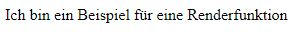
\includegraphics[width=0.5\textwidth]{Theorie/React/Renderfunktion-Ergebnis.png}
    \caption{Ergebnis Renderfunktion}
  \end{center}
\end{figure}

So würde die Renderfunktion von oben dann auf der Website aussehen.


\subsubsection{Komponenten}
In React bestehen die Views aus sogenannten Komponenten. Mit React kann man vordefinierte CodeBits 
programmieren, welche anschließend zu einer View zusammengesetzt werden. Eine React Anwendung 
besteht also aus logisch getrennten Einheiten, die unabhängig voneinander behandelt werden-
Bei React einzigartig ist, dass kein Pattern mit MVC oder MVVM verwendet wird. In React Logik als 
sowohl auch Template in einer JS Datei verwaltet.
HTML-Code wird in React in einer JavaScript Datei geschrieben im sogenannten \textit{JSX-Format}. 
JSX ist HTML jedoch sehr ähnlich.\cite{Komp}


In React gibt es zwei verschiedene Arten eine Komponente zu erstellen.
\begin{itemize}
  \item Komponenten mit State
  \item Komponenten ohne State (Funktionale Komponenten)\\
\end{itemize}

\centerline{\textbf{Komponenten mit State}}
Sie besitzen einen im Konstruktor initialisierten State. Sie sind immer Klassenkomponenten.\\

\centerline{\textbf{Komponenten ohne State}}
Zum Erstellen von Stateless-Komponenten können entweder Funktionen oder Klassen verwendet werden.
Stateless Funktionskomponenten sind vom großen Vorteil und sollten immer verwendet werden, es sei 
denn, man benötigt einen Lebenszyklus-Hook. Stateless Komponenten sind viel einfacher in der
Verwendung.\cite{KompState} 

\subsubsection{JSX}
JSX ist eine syntax Erweiterung zu JavaScript. Es bestimmt wie die Benutzeroberfläche aussehen soll
und erinnert sehr an eine Vorlagensprache. JSX kommt jedoch mit der Kraft von JavaScript. React basiert 
grundlegend darauf, dass die Renderlogik mit der Benutzeroberflächenlogik verbunden wird. JSX ist 
für React nicht notwendig, jedoch ist es ein sehr hilfreiches Werkzeug wenn man in JavaScript-Code an 
der Benutzeroberfläche arbeiten kann. Außerdem ist es sehr hilfreich um Fehler zu finden.
\begin{lstlisting}
  function example jsx(){
    const j = "Hallo, ich bin JavaScript code"

    return(
      <div>
        <p>{j}</p>
      </div>
    )
  }
\end{lstlisting}
Innerhalb der geschwungenen Klammern, kann man jede beliebige Art von JavaScript-Code ausführen.
In diesem Falle würde das $<p>$ Element \textit{Hallo, ich bin JavaScript code} anzeigen.
~\cite{JSX}

\subsubsection{Props}

 Damit die Komponenten in React miteinander kommunizieren können benötigt man Props. Props ist ein
 spezielles Schlüsselwort, welches für Eigenschaften steht und welche man für die Übergabe von 
 Daten von einer Komponente an eine andere verwendet. Daten von Props sollen in nur in eine 
 Richtung weitergegeben werden und zwar vom Elternteil zum Kind. Egal wie eine Komponente 
 deklariert wird, man darf nie ihre Props verändern.\\

 Eine Funktion welche nicht ihre eigenen Eingaben ändert und bei selben Eingaben immer das selben 
 Ergebnis liefert nennt man \textit{pure}.
\begin{lstlisting}
  function sum(a,b){
    return a + b;
  }
\end{lstlisting}
In diesem Beispiel einer pure Function sieht man, dass die Eingabewerte nie geändert werden und egal 
wie oft ich die selben Eingabewerte übergebe, sie werden immer das selbe Ergebnis liefern.


Das Gegenteil einer ``pure Function'' ist eine \textit{impure Function}, welche ihre Eingaben ändert, 
wie man im folgenden Beispiel sehen kann:
\begin{lstlisting}
  function withdraw(account, amount){
    account.total -= amount;
  }
\end{lstlisting}
~\cite{Props}
\pagebreak